%description: Project definition of the Puzzle test-case

\documentclass[letterpaper, oneside]{article}

\usepackage[utf8]{inputenc} 
							
\usepackage[T1]{fontenc}

\usepackage{graphicx} % images
\usepackage{geometry} % margins
\usepackage{latexsym,amsfonts,amssymb, amsmath, amsthm}

\usepackage{subfigure} % several figures
\usepackage{aeguill}  % bitmap fonts ©Ruffin

\bibliographystyle{plain}

%\frenchspacing

\title{Master Thesis -- April/May report}
\date{\today}

\newcommand{\loic}{Loïc Matthey}
\newcommand{\spring}{Spring Berman}

\author{\loic} 

\pagestyle{myheadings} 

% headings
\markright{\loic}

%\addtolength{\textwidth}{1.5cm}
%\addtolength{\hoffset}{-1.5cm}  
%\addtolength{\voffset}{-1.5cm}
%\setlength{\footskip}{0cm}

\begin{document}


%\landscape
\maketitle

% \vspace*{2pt}
% 
% \begin{center}
% \begin{Large}
% 	\textbf{Computational Molecular Biology}\\
% \end{Large}
% \vspace*{5pt}
% \begin{large}
% 	Homework \#7
% \end{large}
% 
% \vspace*{3pt}
% 
% \aut
% 
% \end{center}

%\tableofcontents   % table des matières
%\setcounter{section}{1} 

% Content

\section{Introduction} % (fold)
\label{sec:introduction}
This document presents the current state of the ongoing Master thesis MP12 of Loïc Matthey. This thesis is done in collaboration with the SWIS Laboratory at EPFL, under supervision of Prof. Alcherio Martinoli and the GRASP Laboratory at Penn, under supervision of Prof. Vijay Kumar. We are going to present the work done, precisely define every components of the thesis and discuss what still has to be done.
% section introduction (end)

\section{Project description} % (fold)
\label{sec:project_description}

\subsection{Problem's definition} % (fold)
\label{sub:problem_s_definition}
This thesis aims at answering the following question:

\begin{quote}
Consider an intrinsic complex system with observable dynamics and a measurable performance metric. Let this intrinsic system attains an optimal performance metric value $X_{opt}$. Introduce agents into the system with designed specific behaviors, getting an augmented system. Can we design such behaviors so that the performance metric of the augmented system attains an optimal value $Y_{opt}$, with $Y_{opt} > X_{opt}$?
\end{quote}

We will refer at that question as the \textbf{Intrinsic System Augmentation Problem} (ISAP). We believe that this formulation accurately describe a engineering methodology for different applications. Moreover, we argue that it's easy to represent different problems into that framework. See the note on the Puzzle Test Case for some examples of this reformulation of existing problems \cite{Matthey:2008rm}.
% subsection problem_s_definition (end)

\subsection{General decomposition} % (fold)
\label{sub:general_decomposition}
Starting from the definition of the ISAP, we derived a decomposition into smaller scale components. See Figure~\ref{fig:general_decomposition} for the general decomposition of the problem. See Section~\ref{sub:project_components} for a precise definition of each elements.

\begin{figure}[ht!]
	\centering
		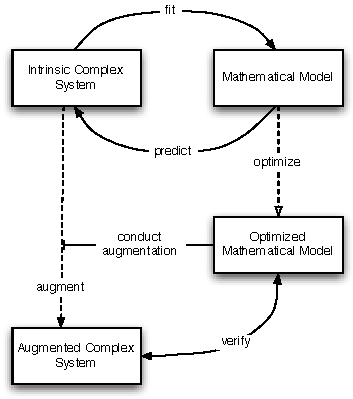
\includegraphics[width=8cm]{img/general_decomposition.pdf}
	\caption{Problem decomposition, top-level components only.}
	\label{fig:general_decomposition}
\end{figure}

Here is the rationale behind it:
\begin{enumerate}
	\item We have an Intrinsic Complex System, that we are able to measure in some way. We will actually present a different formulation of this Intrinsic Complex System, for cases where the real system is not easily measurable, the Compliant Platform. We need to have some insight on this Intrinsic Complex System, because we want to model it mathematically. This is the next step.
	\item We construct and fit a Mathematical Model of this Intrinsic Complex System. We can use this Mathematical Model to predict the Intrinsic Complex System, and will do several iterations to get the best model possible. Different modeling approaches can be taken, as well as simulations strategies for each of them. We concentrate on Chemical Reaction modeling and Stochastic simulation for our framework.
	\item We then take this Mathematical Model and optimize it. This optimization can take a lot of forms, depending on the modeling framework used and the level of plasticity available in the model and initial system. In our project, we will work with Markov Chain optimization, more precisely Fast Mixing-time optimization. This new model can also be simulated, to verify its behavior.
	\item This Optimized Mathematical Model is used to direct the augmentation of the Intrinsic Complex System into an Augmented Complex System. By ``augmented'', we mean modifying the system global behavior using one of some of the following ideas: adding new components, modifying behaviors, modifying components. This is a Top-down approach to complex system control. Once we know how to augment the intrinsic system, we have to verify that it indeed behave like the optimized model. Hence we perform several iterations of the augmentation, so that the optimized mathematical model actually captures the new Augmented Complex System.
	\item We can then study the Augmented Complex System, to see what was changed for it to behave better. This could give insight in processes that are hard to study, especially when taking the Compliant Platform approach.
\end{enumerate}

These top-level components can be divided into more precise components, as shown in the next section.
% subsection general_decomposition (end)

\subsection{Project components} % (fold)
\label{sub:project_components}

\subsubsection{Intrinsic Complex System} % (fold)
\label{ssub:intrinsic_complex_system}

See Figure~\ref{fig:img_intrinsic_complex_system} for the diagram. This component represent the actual system we want to study and optimize. There are two possibilities for this component:

\begin{figure}[h!]
	\centering
		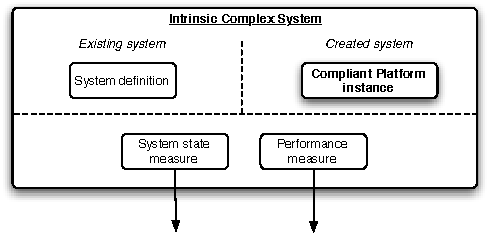
\includegraphics[width=11cm]{img/intrinsic_complex_system.pdf}
	\caption{Intrinsic Complex System component. Black arrows show inter-component communication, with other top-level components. Compliant Platform Instance in bold is defined in another diagram.}
	\label{fig:img_intrinsic_complex_system}
\end{figure}

\begin{description}
	\item[Existing system:] In that case, we have a complex system already existing. Such applications could be existing platforms for self-assembly, or an existing natural process. We need to be able to measure the state of this system in some way, as well as assessing its performance according to a desired metric. These informations are then used by the Mathematical Model component or to assess the performance of the system.
	\item[Created system:] If we do not have a complex system to observe, or if the actual complex system is not measurable, we can bypass that by \textbf{creating} an intrinsic complex system. For that we introduce a \textbf{Compliant Platform instance}.
\end{description}

A Compliant Platform is a real or simulated platform allowing a big variety of problems reproduction. The aim is to propose a set of agents that can reproduce any given problem compatible with their hardware capabilities. We chose to use a robotic platform for that. The robots can simulate manipulation, assembly and coordination tasks, at a scale where measurability is not a problem. We want then to create an instance of this Compliant Platform to reproduce a desired complex system. Such a targeted complex system could be a biological pathway, a self-assembly process, or, in our case, a puzzle building task. The Compliant Platform can ensure that some properties are met. Such a condition is the well-mixed property, which we will use in our puzzle test-case.

The description of the Compliant Platform instance is shown in Figure~\ref{fig:img_compliant_platform_instance}.

\begin{figure}[h!]
	\centering
		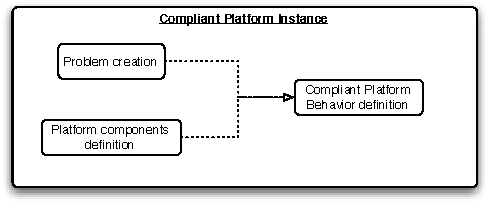
\includegraphics[width=11cm]{img/compliant_platform_instance.pdf}
	\caption{Compliant Platform Instance component. Dotted arrows show termination dependencies between components.}
	\label{fig:img_compliant_platform_instance}
\end{figure}

\begin{itemize}
	\item The first step is to actually create a problem we want to reproduce. This is actually a complicated task, as we might already restrict the scope of the problem at this very early step. Different choices can be made, but they have to be in accordance with the Model optimization used in the Optimized Mathematical Model component. For our current project, we assume the following strategy: the Model optimization performs a continuous optimization of reaction rates. If we need a discrete optimization, this should be done beforehand at the Problem creation stage (the discrete parts are the reactions considered).
	\item The second needed thing is a definition of the platform capabilities. A complete Compliant Platform should provide the following actions for the agents presents in the platform:
		\begin{enumerate}
			\item Movement capabilities.
			\item Interactions, locally and more globally.
			\item Combination/assembly.
			\item Creation.
			\item Destruction.
		\end{enumerate}
	For example, when reproducing a biological process like protein translation, we would need the following actions: Movement, Interactions, Combination, Creation and Destruction. For our current project, which studies assembly, we only need Movement, Interactions and Combination.
	The current Compliant Platform we are developing aims at reproducing the assembly process, so we do not offer all possibilities for now. This is a possible further work for next iterations.
	\item When we know what to reproduce and what are the capabilities of the agents, we need a description of the task to perform. We call this a Compliant Platform Behavior, and this can take any format. For now, we assume that such a behavior consists in a robot controller. A potentially interesting improvement is to write the behavior as a set of reactions channels. This would allows a direct translation of known chemical or biological processes for people more used to this notation. The platform would then have to reproduce this set of reactions if possible. 
\end{itemize}

% subsubsection intrinsic_complex_system (end)

\subsubsection{Mathematical model} % (fold)
\label{ssub:mathematical_model}

The Mathematical model component aims at reproducing as well as possible the Intrinsic Complex System, while being quicker to simulate. See Figure~\ref{fig:img_mathematical_model} for the diagram of this component.

\begin{figure}[h!]
	\centering
		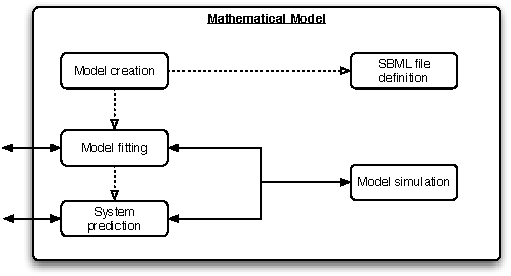
\includegraphics[width=11cm]{img/mathematical_model.pdf}
	\caption{Mathematical Model component. Black arrows show inter-component communication. Dotted arrows show termination dependencies between components.}
	\label{fig:img_mathematical_model}
\end{figure}

\begin{itemize}
	\item The first step is to \textbf{create the model}. This creation consists on the choice of a modeling notation and depends on the knowledge we have about the system. We propose to use a \textbf{Chemical Network} notation for this component. A Chemical Network notation is mainly used by chemist to show networks of coupled biochemical reactions. This level of representation is at the same time very general, offering representation of very different processes, and also quite precise and detailed, allowing to construct full dynamic simulations of the system behavior on a computer.
	Adapted from \cite{Wilkinson:2006yg}:
	
	\begin{quote}
		A general chemical reaction takes the form
		\[
			m_1 R_1 + m_2 R_2 + \ldots + m_r R_r \xrightarrow{} n_1 P_1 + n_2 P_2 + \ldots + n_p P_p
		\]
		where $r$ is the number of reactants and $p$ the number of products. $R_i$ is the $i$th reactant molecule and $P_j$ the $j$th product molecule. $m_i$ is the number of molecules of $R_i$ consumed in a single reaction step, and $n_j$ the number of molecules of $P_j$ produced. The coefficients $m_i$ and $n_j$ are known as \emph{stoichiometries}. If we assume mass-action stochastic kinetics, we also associate with each reaction a \emph{stochastic rate constant} $c_i$ and an associated \emph{rate law} (also \emph{hazard} or \emph{propensity} function) $h_i(x,c_i)$. $x$ is the current state of the system.
		This allows then to simulate exactly the modeled process assuming we know all the rate constants and rate laws.
	\end{quote}
	A very advanced further work is the possibility to automatically create the model, using some model discovering scheme (navigating through the models space). This is most likely a very hard problem, and we do not consider it for now.
	\item We will save this Chemical Network model in a specific standardized format: System Biology Markup Language (\textbf{SBML}) \cite{Hucka:2003qd}. This is a XML-based file format designed to store systems of chemical reactions. As this seems to be a standard in the community and because some tools are already available to handle it, we will use that format as a common definition of our mathematical models. We will use \emph{libSBML} \cite{Bornstein:2008hl} to load and handle SBML files. We assume as of now that this model will be automatically updated according to further refining.
	\item The model has to be fitted in some way to the Intrinsic Complex System. If we are using an existing complex system, then this is a quite complex problem, especially if we do not have precise insight in the behavior of the system. We can use methods like Bayesian Inference or MCMC (Markov Chain Monte Carlo) to fit the model on the experimental data. If we are using the Compliant Platform, than we assume that we can measure much more precisely the processes taken place, and this model fitting is more straightforward.
	\item To be able to fit the model, we need to actually see how well it fits. So we need a \textbf{simulation framework} for the mathematical model. As we use a Chemical Network modeling framework, we have existing theory to rely on. Several possibilities exists to simulate a Chemical Network:
	\begin{enumerate}
		\item The simplest one is to use an \textbf{ordinary differential equation} (ODE) simplification. This is the level used by chemistry for process which are well-mixed. Common ODE solving strategies can be used to simulate that. We will use Matlab for this purpose.
		\item As the processes we study are intrinsically stochastic and do not correspond to the scales used usually by chemists (thermodynamic limit), we want to study how a \textbf{stochastic simulation }performs. We can use an exact simulation, like Gillespie's Stochastic Simulation Algorithm, or other derivatives (Gibson \& Bruck, $\tau$-leaping).
		\item We will also consider using \textbf{hybrid simulations} schemes, namely simulations which mix stochastic components and deterministic approximations, based on the existence of multi-scale dynamics. Different possibilities exist here also, like stochastic-ODE simulation, multi-scale $\tau$-leaping and many others.
	\end{enumerate} 
	We will implement those simulations in Matlab, using available tools if possible. They will all need as input a SBML file describing the model.
	
	\item We can then run our mathematical model to predict the system's behavior. Comparing that with the actual behavior of the system and trying to improve the fitting gives a iterative process to improve the model. Furthermore, we can then use the model to test hypothesis and performs experiments at a much higher speed than using directly the complex system (this is the rational behind a multi-level modeling framework).
\end{itemize}

% subsubsection mathematical_model (end)

\subsubsection{Optimized Mathematical model} % (fold)
\label{ssub:optimized_mathematical_model}

When the mathematical model represents the intrinsic complex system correctly, we will then use it to improve the initial complex system. As the model is easier to manipulate and based on mathematical concepts which can be modified easily, we think it is easier to perform the optimization at this level. Moreover, we will use optimizations scheme that work ``blindly'', that is which have no insight into the system concepts, and thus which will not make bad assumption as one human could do.

We will then need to map the new mathematical model onto the complex system, a step we call system augmentation. This is a Top-down optimization approach, which we think is more appropriate for the kind of complex systems we are handling. This makes even more sense if we do not know a-priori how to change the behavior of the intrinsic complex system, because of its complexity. Working on the model level gives another level of abstraction that helps to understand the acting processes of the complex system.

See Figure~\ref{fig:img_optimized_mathematical_model} for this component's diagram. 

\begin{figure}[h!]
	\centering
		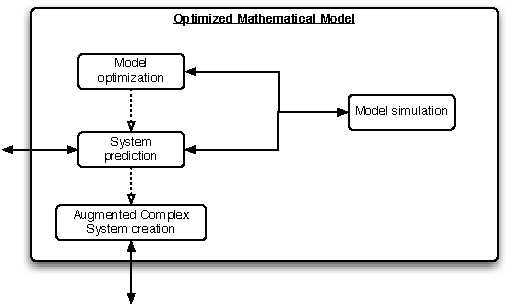
\includegraphics[width=12cm]{img/optimized_mathematical_model.pdf}
	\caption{Optimized Mathematical model component. Black arrows show inter-component communication. Dotted arrows show termination dependencies between components.}
	\label{fig:img_optimized_mathematical_model}
\end{figure}

\begin{enumerate}
	\item The first step is to actually \textbf{optimize the model}. As we already said before, this step should be in accordance with the problem creation we chose when starting. We assume for our project that we will perform a continuous optimization. Endless ways of optimizations exists, depending on the model chosen or desired goals. As we are working with Chemical Networks and interested with stochastic processes, we will perform an optimization using a Markov Chain paradigm. It fits well our puzzle test-case which replicate an assembly process.
	
	We represent the reactants and products as a Markov Chain, with transitions according to available reactions. The goal is to optimize the yield. That is, we want to get as much final product $P_f$ as possible, as quickly as possible. We will perform that by reducing the problem to a Fast Mixing Time Markov Chain problem. We need to optimize the time of mixing of a markov chain, under the constraint that the stationary distribution of that chain represents the state with a maximal yield of product $P_f$.
	
	Problems could arise, as we are working with inhomogeneous Markov Chains (reactions kinetics can be non-linear). Moreover, it needs to be a scalable approach and easy to apply to different test cases. We will need to assess its applicability. But this optimization scheme, if working correctly, is completely general, independent of the underlying process and could gives us additional insight into the complex system. For example, assuming we are optimizing an assembly process, optimizing the time to mixing should hypothetically optimize the parallelism of the reactions also.
	\item This optimization will extensively use the model simulation framework we built, to assess the new performance.
	\item We then again use that new optimized model to predict the behavior of the system, and to possibly gain insight into the system's behavior.
	\item The last and quite difficult part of this component is to use the optimized model as a guideline to the \textbf{augmentation of the intrinsic complex system}. This is a Top-down mapping problem, where we need to transfer the modifications done in the model onto the complex system, so as they match closely. We will iterate several times, to map as closely the new Augmented Complex System onto the Optimized mathematical model.
\end{enumerate}
% subsubsection optimized_mathematical_model (end)

\subsubsection{Augmented Complex System} % (fold)
\label{ssub:augmented_complex_system}

This last component is the actual realization of the mathematical model we optimized. As we said, we want to modify the intrinsic complex system so that we obtain higher performances. We will use the optimized mathematical model and try to inverse the modeling process: modify the complex system so that it behaves like the model. See Figure~\ref{fig:img_augmented_complex_system} for the component's diagram.

\begin{figure}[h!]
	\centering
		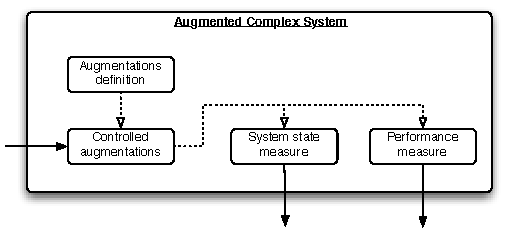
\includegraphics[width=12cm]{img/augmented_complex_system.pdf}
	\caption{Augmented Complex System model component. Black arrows show inter-component communication. Dotted arrows show termination dependencies between components.}
	\label{fig:img_augmented_complex_system}
\end{figure}

\begin{enumerate}
	\item First of all, we need to define what can be changed or added in the intrinsic complex system. This is a hard task because we might not know what to add or modify into the intrinsic complex system to create the modified dynamics. We could allow list of actions, assessing their effects on the model, or try to discover automatically ways of changing the behavior of the complex system. This is the most open question in our framework, and more thinking is needed on that.
	\item When we know what can be changed, we will explore the possibilities, following the guidelines given by the Optimized mathematical model. We need to measure the system state for that, as well as measure the obtained performance.
	\item The final step will be to assess the applicability of this Top-down optimization scheme, and see if it is a valid and general enough idea.
\end{enumerate}

% subsubsection augmented_complex_system (end)
% subsection project_components (end)

\subsection{Test cases} % (fold)
\label{sub:test_cases}

We will extensively verify the applicability of our problem definition and solving on different test cases. They should represent different systems and different scales, to verify when and how our framework is applicable.
\subsubsection{Puzzle Test case} % (fold)
\label{ssub:puzzle_test_case}
Our first test case is an idealization of an assembly task. Further informations are available in a specific note \cite{Matthey:2008rm}. The general idea is to assemble different pieces into a defined shape. Pieces can assemble using determined anchoring points. The goal is to assemble as many puzzles as possible given an initial population of pieces.

This can be made more interesting by allowing mistakes in the connections, or by trying to create the final shape while knowing only partial information on the assembly plan.

This test case also aims at studying the applicability of using very simple stochastic assembly versus more heavy controlled assembly.
% subsubsection puzzle_test_case (end)

\subsubsection{Self-assembly case} % (fold)
\label{ssub:self_assembly_case}
We will model a self-assembly task at the nanoscale level. This will use either the work of G. Mermoud on MEMS, or the work of N. Ayanian on dry self-assembly.
% subsubsection self_assembly_case (end)

% subsection test_cases (end)
% section project_description (end)


\section{Puzzle test-case state} % (fold)
\label{sec:puzzle_test_case_state}

We present the actual work done on the Puzzle test-case. A formal definition of the test-case was done in \cite{Matthey:2008rm}. The definition of the two controllers considered as changed since that time, so we present the new definition.

\subsection{Puzzle assembly task} % (fold)
\label{sub:puzzle_assembly_task}
\begin{itemize}
	\item Let a puzzle of square shape, with area $25$, be constructed out of 5 pieces of area 5 each with different given shapes.
	\item Let the final assembly shape $S$ of this puzzle be know.
	\item Let the set of assembly plans $P$ leading to the final shape $S$ be known. 
	\item Let the puzzle pieces assemble by bi-directional connections. One connection is enough for two pieces to be attached. These connection and their positions on the different pieces are known.
	\item Pieces can be assembled and disassembled.
	\item Consider an arena of sufficiently large size so that small scale interactions dynamics can be ignored.
	\item Fill this arena with $N$ initial pieces of each shape.
	\item Consider $M$ robots, able to pick up pieces and to make them assemble and disassemble.
	\item Allow a recognition by the robots and by the pieces of the shapes and connection points when an encounter occur.
	\item \textbf{Then:}\\
	How can you manipulate those initial pieces so that after a time $T_f$, the number of assembled puzzles $X_S$ is maximized?
\end{itemize}

We then have a lot of different possibilities for the robot behaviors. We chose to consider different directions depending on the available information and capabilities of the robots. If we want to produce something really scalable, then using robots as simple as possible is interesting. But on the other hand, it could come with a too big impact on the performances. So we will try to measure this with respect to several considerations.

\begin{table}[h!]
	\begin{center}
	\begin{tabular}{r|c|c}
		& \textbf{Assembly plan known} & \textbf{Local plans only} \\
		\hline
		\textbf{Local information} & \emph{Current study} & \emph{Future work} \\
		\hline
		\textbf{Global information} & Market-based, Assembly line & Market-based
	\end{tabular}
	\end{center}
	\caption{Robot behavior depending on available informations.}
	\label{tab:robot_behavior}
\end{table}

The first distinctions we make are shown in Table~\ref{tab:robot_behavior}. The most important criteria is the availability of information about the robots and pieces positions and states. If we have a Global information state, then the problem reduces to a classical assembly at the macro-level. With multiple robots, this could be solved using Market-based strategies, which do not interest us here. So we only consider having Local information about the pieces and robots positions.

The next distinction is the availability of the full assembly plan. Knowing the full assembly allows to optimize a-priori a plan and to stick to it when building the puzzle. But this needs some computing capabilities and communications between pieces and robots. A more crude possibility is forbidding this full knowledge, and having to recreate the global plan only from local connections possibilities.

We are currently studying the \emph{Local info/Assembly plan} case. We also plan to study, if times allows, the \emph{Local info/Local plan} case.

Furthermore, we have the following choice to make: \emph{should the pieces be disassembled or not}?
As we will develop during the project, this depends on the possibility of bad assemblies and bad recognitions. This is then a trade-off between robustness to noise and efficiency (as obviously sticking to a direct application of the optimal plan should be better than doing wrong assemblies).

Please note that when the study of the \emph{Local info/Local plan} case, we may find a way to tackle both problems using the same strategy. Indeed, both problems emerges from limited knowledge of the system state.
% subsection puzzle_assembly_task (end)	

\subsection{Webots implementation} % (fold)
\label{sub:webots_implementation}

We created the defined problem using Webots. It allows us to get a realistic simulation of an assembly. According to our formulation, we are creating a Compliant Platform using Webots.

\subsubsection{Pieces} % (fold)
\label{ssub:pieces}

We modeled the pieces in Webots, as CustomRobots. We use Connectors to simulate magnets for the assembly of the pieces. They have an emitter/receiver to communicate with the carrying robots.

Pieces connect to each other using magnets on their sides, and are carried around by the robots using the magnet on their top.

See Figure~\ref{fig:img_assembly_plan} for a view of the different pieces, their connections points and the final puzzle to construct.

\begin{figure}[h!]
	\centering
		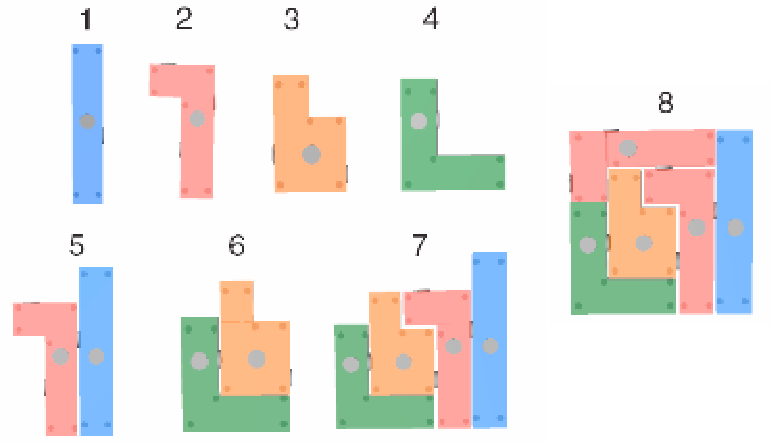
\includegraphics[width=12cm]{img/assembly_plan.pdf}
	\caption{Pieces constructed and the actual plan to construct the final assembly. Courtesy of S. Berman.}
	\label{fig:img_assembly_plan}
\end{figure}
% subsubsection pieces (end)

\subsubsection{Robots} % (fold)
\label{ssub:robots}


For the robots, we used the KheperaIII model available in Webots. It offered a small scale yet not too crude mobile robot for our first implementation. We plan on modeling the Scarab robots, used at the GRASP Laboratory, for further experiments.

\begin{figure}[h]
	\centering
		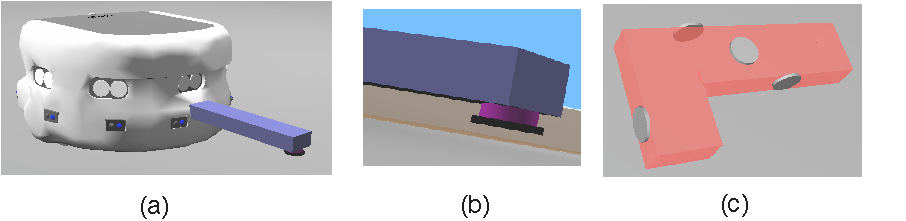
\includegraphics[width=14cm]{img/SimSetup.pdf}
	\caption{Simulation platform.  (a) Khepera III robot with carrying arm; (b) close-up of arm, with mobile Connector; (c) puzzle piece. Courtesy of S. Berman.}
	\label{fig:img_SimSetup}
\end{figure}

In order to manipulate the pieces, we equipped the robots with a protruding carrying arm (see Figure~\ref{fig:img_SimSetup}). This arm consists of a simple bar with a mobile Connector at its end. The Connector is allowed to turn around 360$^{\circ}$ using a rotational Servo, in order to orient the carried piece in the right direction. The length of the arm should be sufficient to rotate any mid-assembly without hitting the robot's body.

When being carried, the piece does not touch the ground, as they are very light-weight. This can be modified, but in earlier simulations, it created some problems in Webots, with unrealistic moments that disrupted the plausibility of the physical simulation.
% subsubsection robots (end)

\subsubsection{Obtained assembly behavior} % (fold)
\label{ssub:obtained_assembly_behavior}
For her final project in the Advanced Robotics course (MEAM 620), S. Berman implemented a working assembly task in Webots using the pieces and robots presented before. The behavior, shown in Figure~\ref{fig:behavior_webots_assembly}, is as follows:

\begin{itemize}
	\item Pieces and robots are placed randomly in the arena.
	\item Robots move around, searching for lying pieces. For the project, the robots moved forward, avoiding the wall using a Braitenberg vehicle controller. We changed this movement later to ensure well-mixing of the pieces. See Section~\ref{ssub:movement_pattern_of_robots} for the results.
	\item Robots and pieces broadcast messages locally, telling their ID and current state.
	\item When a robot encounter a free piece, it aligns with it, go to it and carries it. This alignment uses relative range and bearing offered by the emitter/receiver nodes of Webots.
	\item According to the piece type and the assembly plan, the robot then orient it so as to show the good Connector in front. Again we use the relative range and bearing of emitter/receiver nodes to perform that alignment.
	\item While carrying the piece, the robot start moving around again, searching for another robot with a compatible piece. Robot communicate with small range messages broadcasted at all time. They look into their assembly plan when encountering another robot with a piece, and if nothing corresponds, it moves away from it.
	\item When another compatible robot is encountered, they align themselves and start the approach. Then one of the robot leaves, leaving the other one with the assembled pieces. This robot then align its piece and start searching for another robot with a compatible piece, for the new assembly. If the obtained piece is the final assembly, the robot drops it on the floor.
\end{itemize}

The next step is to make this implementation more robust and scalable, although now some error checking is already working.

\begin{figure}[h]
	%\centering
	\subfigure[Robot searching pieces] 
	{
		\label{fig:img_search_piece}
		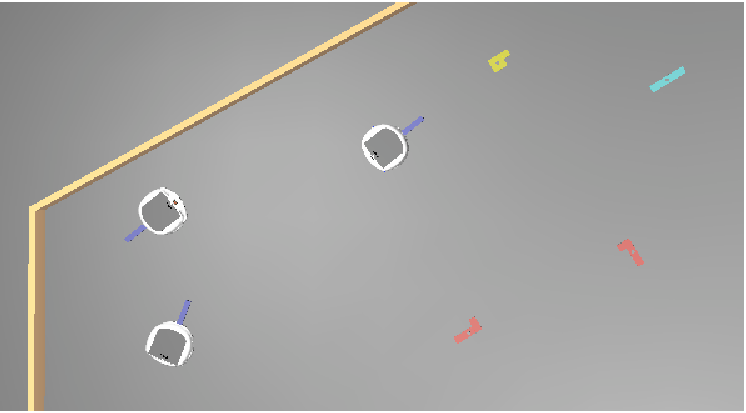
\includegraphics[width=8cm]{img/search_piece.pdf}
	}
	\; % espacement entre figures. \quad \;
	\subfigure[Encountering between a robot and a piece] 
	{
		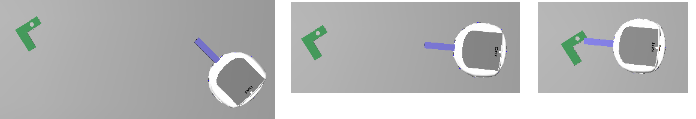
\includegraphics[width=8cm]{img/align_approach_piece.png}
		\label{fig:img_align_approach_piece}
 	}
	\; % espacement entre figures. \quad \;
	\subfigure[Alignment of piece by the rotating connector] 
	{
		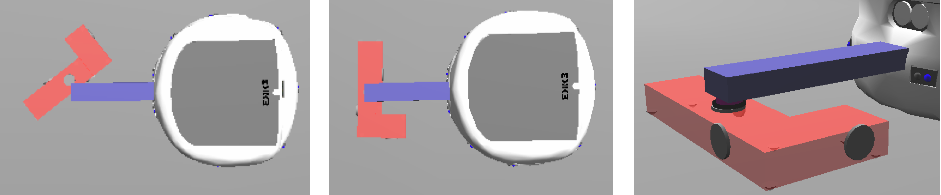
\includegraphics[width=8cm]{img/rotate_piece.png}
		\label{fig:img_rotate_piece}
 	}
	\; % espacement entre figures. \quad \;
	\subfigure[Approach between two robots] 
	{
		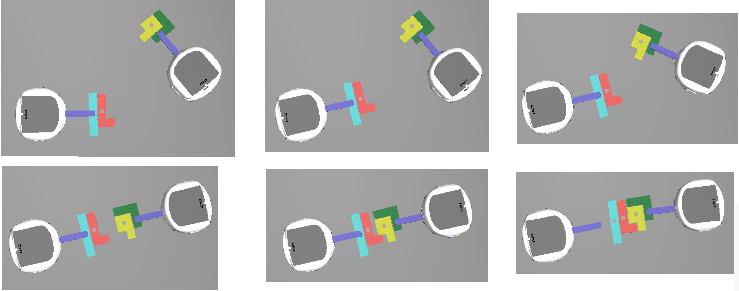
\includegraphics[width=8cm]{img/align_approach.png}
		\label{fig:img_align_approach}
 	}
	\caption{Behavior in the current Webots assembly world. Courtesy of S Berman.}
\label{fig:behavior_webots_assembly} %Cation general
\end{figure}

We need now to measure this system, and see if we can model it using Chemical Networks accurately, like we want to do.
% subsubsection obtained_assembly_behavior (end)

\subsubsection{Movement pattern of robots} % (fold)
\label{ssub:movement_pattern_of_robots}
One of the thing we want to enforce for the assembly test-case is the well-mixing property of pieces. That way, we are replicating a solution with randomly moving components.

The first controller we implemented just made the robots go forward, while avoiding the walls and other robots.

We then developed a new controller, which moved according to a bacterial-like movement. This movement, ``chemotaxis'', allows bacteria to move around, search for nutriments and avoid dangers. It is based on a forward movement, and random ``tumbling''. A ``tumble'' is a random turn. The bacteria sample the concentration of nutriments or dangerous chemicals, and performs a temporal integration on them while moving. An increase in a nutriments concentration tends to reduce the number of tumbling, promoting movement towards the spacial gradient. When the gradient is constant, the bacteria performs tumbling at a constant rate \cite{Adler:1975p7745}\cite{Macnab:1972p7813}.

In our case, we do not follow any gradient. We only make the robots move forward for a random distance, and then turn randomly around, before moving forward again. This creates a random movement that is thought to cover more uniformly the space.

To assess both controllers performances, we derived a measure protocol.
We sample the positions of 5 robots moving in the hexagonal arena. We perform 5 runs of 10 simulated minutes each. The robots are positioned randomly initially. The goal is to cover the arena the more uniformly as possible. The coverage is the average time passed in a specific position. We derived a metric to assess the coverage quality, see Equation \eqref{eq:coverage_error}.
\begin{equation} \label{eq:coverage_error}
	E = \sum_{\{x,y\} \in arena}|c(x,y) - p(x,y)|
\end{equation}

where $E$ is the error of coverage, $c(x,y)$ is the average time passed in position $(x,y)$ and $p(x,y)$ is the perfect theoretical coverage, with uniform distribution on the whole arena.
Both controller performances are shown in Table~\ref{tab:error_coverage} and the visual coverage is shown in Figure~\ref{fig:covering_controllers}. 

\begin{table}[h!]
	\begin{center}
	\begin{tabular}{|c|c|}
		\hline
		\textbf{Controller} & \textbf{Error} \\
		\hline
		Forward & 0.762 \\
		\hline
		Bacterial & 0.274 \\
		\hline
	\end{tabular}
	\end{center}
	\caption{Error of coverage according to \eqref{eq:coverage_error}, for both robot controllers.}
	\label{tab:error_coverage}
\end{table}


\begin{figure}[h!]
	\centering
	\subfigure[Forward controller, 3D] 
	{
		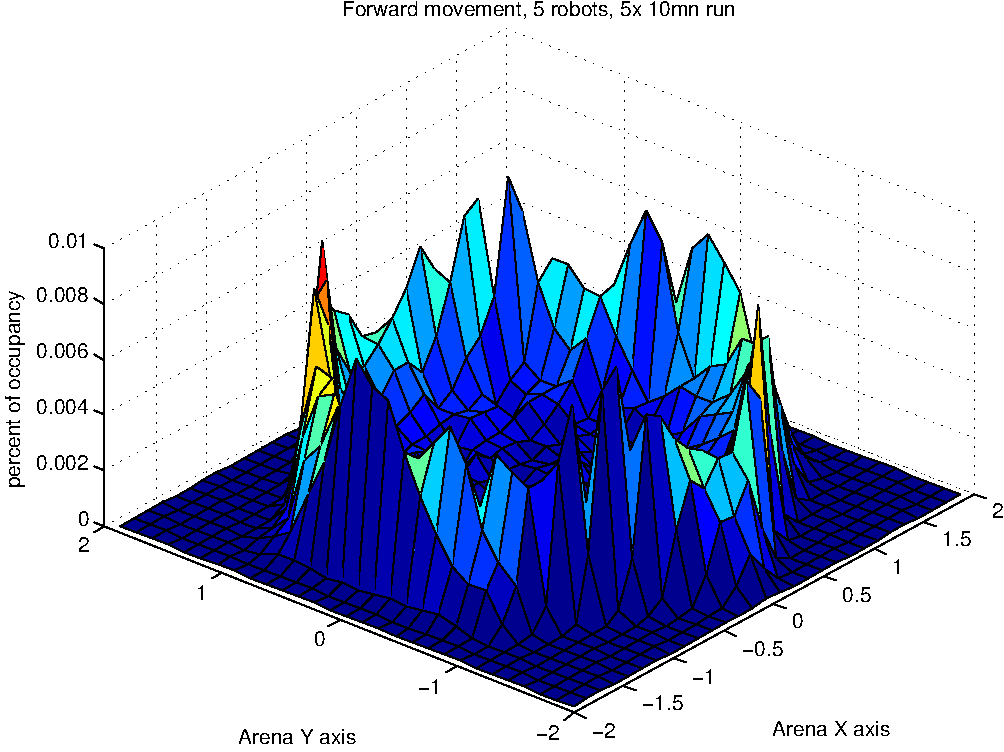
\includegraphics[width=6cm]{img/forward_covering_3d.pdf}
		\label{fig:img_forward_covering_3d}
	}
	\; % espacement entre figures. \quad \;
	\subfigure[Forward controller, 2D] 
	{
		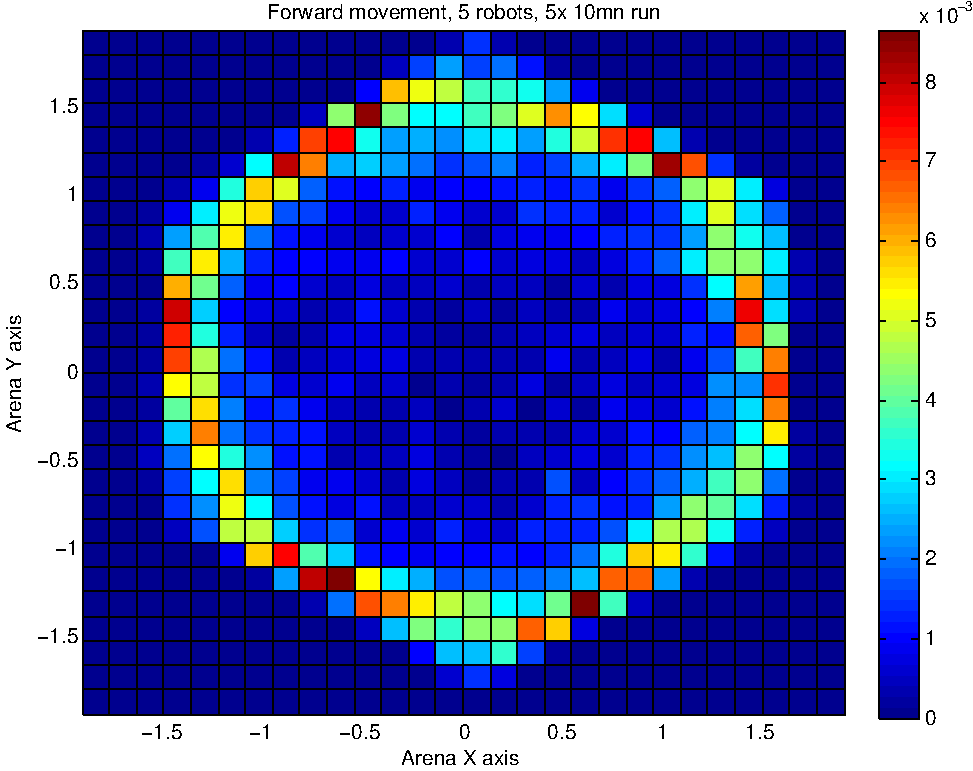
\includegraphics[width=6cm]{img/forward_covering_2d.pdf}
		\label{fig:img_forward_covering_2d}
 	}
	\\ % espacement entre figures. \quad \;
	\subfigure[Bacterial controller, 3D] 
	{
		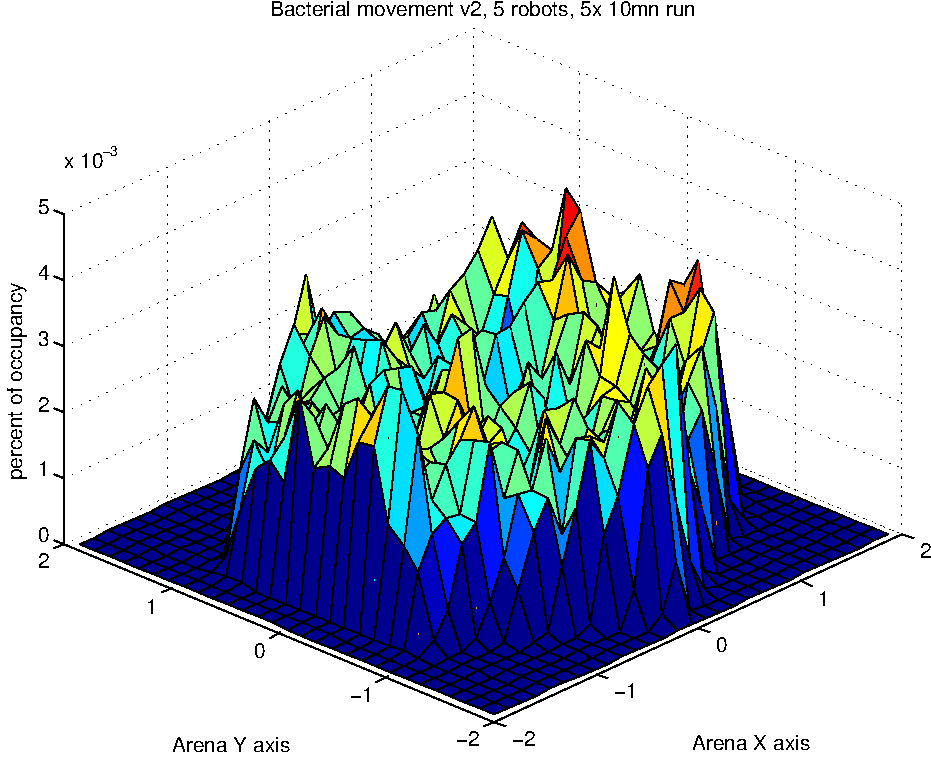
\includegraphics[width=6cm]{img/bacterial_covering_3d.pdf}
		\label{fig:img_bacterial_covering_3d}
 	}
	\; % espacement entre figures. \quad \;
	\subfigure[Bacterial controller, 2D] 
	{
		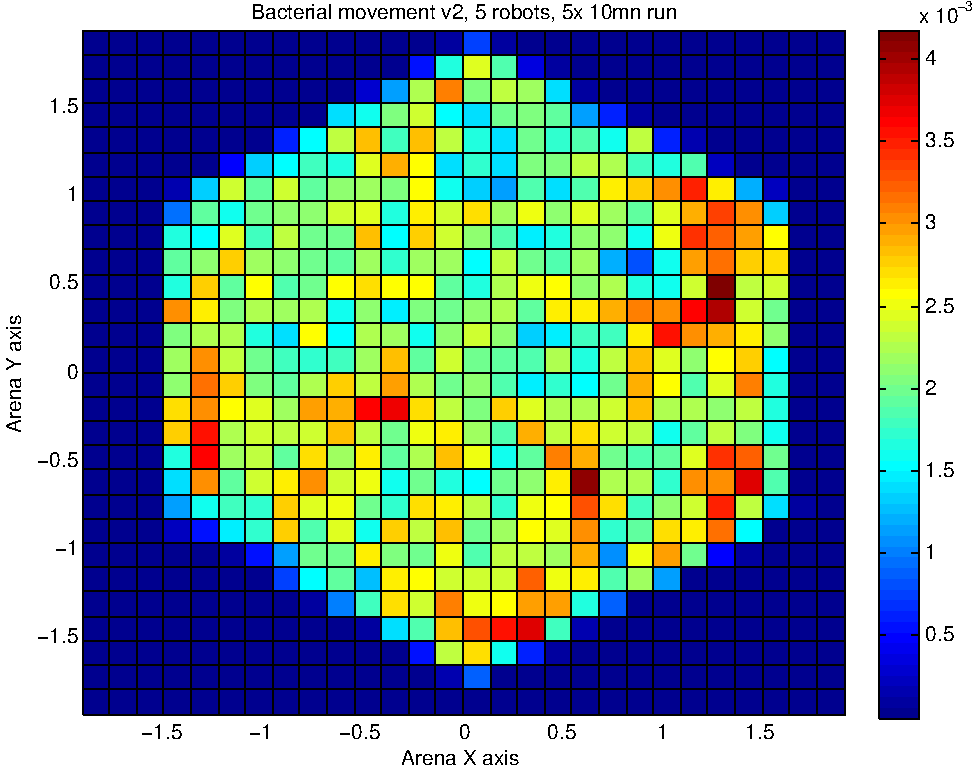
\includegraphics[width=6cm]{img/bacterial_covering_2d.pdf}
		\label{fig:img_bacterial_covering_2d}
 	}
	\caption{Average coverage of the arena by 5 robots for two different controllers.}
\label{fig:covering_controllers} %Cation general
\end{figure}

We see that with the forward controller, the robots were moving on a circle, which is not well-mixed at all. The bacterial controller, on the other hand, performs a really good distribution over the whole arena. Our metric accurately shows that. We thus stick to the bacterial movement from now.

% subsubsection movement_pattern_of_robots (end)
% subsection webots_implementation (end)

\subsection{Webots Python World Generator} % (fold)
\label{sub:webots_python_world_generator}
In order to create Webots worlds containing a big number of pieces of robots, we decided to create a separate world generator. We implemented it in Python. The generator takes a world description file written in XML, and generate a world according to it.

Currently, we support the following components:

\begin{description}
	\item[Arena:] Generate a square or hexagonal arena, of desired radius.
	\item[Pieces:] Position a desired number of pieces in specific or randomly chosen positions within the arena, while trying to avoid overlap between them. The pieces are taken from a library of templates. We can specify the desired controller that the pieces should use.
	\item[Robots:] Position a desired number of robots in specific or randomly chosen positions within the arena, while trying to avoid overlap between them. Robots can be KheperaIII with or without the carrying arm, according to a library of templates. The controller can be specified.
	\item[Supervisor:] Create a Supervisor, with a specific controller.
\end{description}

Further components and extensions will be added during the project.

This program is distributed under a GNU Lesser General Public Licence, and is available on the Yahoo! Mailing List of Webots.
% subsection webots_python_world_generator (end)

% section puzzle_test_case_state (end)

\section{Webots self-assembly world} % (fold)
\label{sec:webots_self_assembly_world}

\begin{figure}[h!]
	\centering
		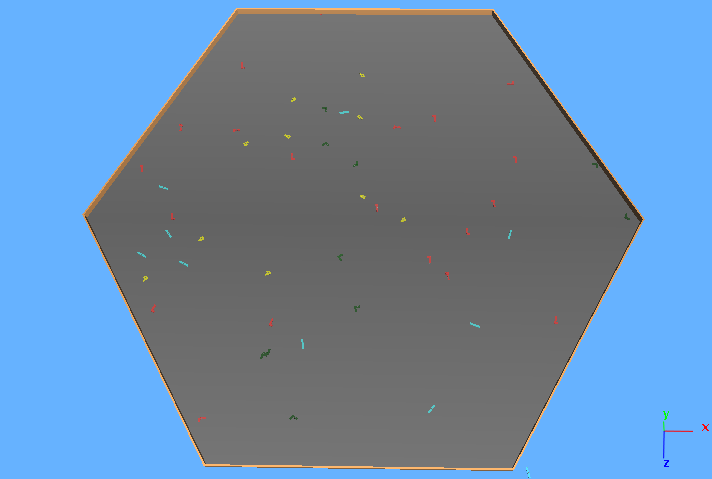
\includegraphics[width=9cm]{img/webots_self_assembly_random.png}
	\caption{Self-assembly Webots world}
	\label{fig:img_webots_self_assembly_random}
\end{figure}

When starting the project, we created a simple self-assembly demonstration using Webots. This world consists of a defined number of pieces, the same one that were used in the Puzzle test-case. We will still keep it as an potential test case for self-assembly, as it involves less components and computations.

The pieces move around randomly, pushed by random forces. These forces are independent of each others, so this is not a simulation of a mixed liquid. This could be an interesting modification, using a physic plugin in Webots.
% section webots_self_assembly_world (end)

\section{Further work} % (fold)
\label{sec:further_work}
Further work include creating all components shown in Section~\ref{sec:project_description} and not already realized.

We already have a intrinsic complex system, namely the Puzzle test-case (and also the self-assembly world), which we can measure and modify the behavior. We will continue to research possible directions for solving the assembly problem while errors arise.

The most important part now is the simulation platform, which will allows us to model the Puzzle test-case and determine what kind of simulation precision is needed for such problems.

We will then study the optimization scheme and see if it can be applied to problems with nonlinear dynamics.
% section further_work (end)

\bibliography{report_april}

\end{document}
